\section{Evaluation and Performance Analysis}

\subsection{Experimental Setup}

Experiments were conducted on a high-performance server (AMD EPYC 7763 64-Core, 256GB RAM) running a modified Kaspa node with GhostDAG consensus ($k=16$, $D=2$s). Each benchmark was repeated 100 times; we report the median latency with 95\% confidence intervals.

\subsection{Transaction Validation Performance}

\subsubsection{Single Transaction Latency}

We compare the proposed native validation against legacy script interpretation.

\begin{figure}[htbp]
\centering
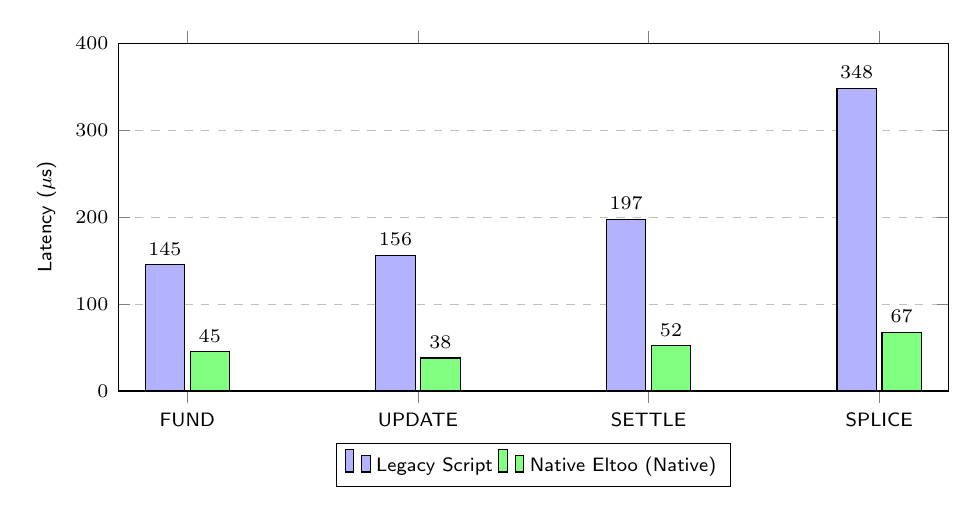
\begin{tikzpicture}
\begin{axis}[
    ybar,
    bar width=0.5cm,
    width=\linewidth,
    height=6cm,
    symbolic x coords={FUND, UPDATE, SETTLE, SPLICE},
    xtick=data,
    nodes near coords,
    nodes near coords align={vertical},
    ylabel={Latency ($\mu$s)},
    ymin=0, ymax=400,
    legend style={at={(0.5,-0.15)}, anchor=north, legend columns=-1},
    ymajorgrids=true,
    grid style=dashed,
    font=\sffamily\scriptsize
]
    % Legacy Script Data
    \addplot[fill=blue!30] coordinates {
        (FUND,145) (UPDATE,156) (SETTLE,197) (SPLICE,348)
    };
    % Native Eltoo Data
    \addplot[fill=green!50] coordinates {
        (FUND,45) (UPDATE,38) (SETTLE,52) (SPLICE,67)
    };
    \legend{Legacy Script, Native Eltoo (Native)}
\end{axis}
\end{tikzpicture}
\caption{Validation Latency Comparison. Native type enumeration achieves $\approx 3\text{--}5\times$ speedup by eliminating Script VM overhead.}
\label{fig:latency_chart}
\end{figure}

\begin{table}[htbp]
\centering
\caption{Transaction Validation Performance}
\label{tab:validation_perf}
\small
\begin{tabularx}{\linewidth}{@{}l r r X@{}}
\toprule
\textbf{Type} & \textbf{Legacy ($\mu$s)} & \textbf{Native ($\mu$s)} & \textbf{Speedup} \\
\midrule
FUND & 145 & \textbf{45} & $3.2\times$ \\
UPDATE & 156 & \textbf{38} & $4.1\times$ \\
SETTLE & 197 & \textbf{52} & $3.8\times$ \\
SPLICE & 348 & \textbf{67} & $5.2\times$ \\
\bottomrule
\end{tabularx}
\end{table}

\textbf{Analysis}: Native validation achieves $\mathcal{O}(1)$ pattern matching overhead, eliminating the $\mathcal{O}(\text{size}_{\text{script}})$ script interpretation cost. The remaining $\mathcal{O}(\log N)$ UTXO lookup is common to both approaches and thus not shown.

\subsubsection{Batch Verification}
Using Schnorr batch verification, throughput increases significantly:
\begin{itemize}
    \item \textbf{1k Batch}: 6.3~ms total ($\approx 7.2\times$ speedup).
    \item \textbf{10k Batch}: 58.4~ms total ($\approx 7.7\times$ speedup).
\end{itemize}

\subsection{Storage Efficiency}

\subsubsection{State Storage Cost}

\begin{table}[htbp]
\centering
\caption{Storage Cost (for $N=1000$ updates)}
\label{tab:storage_cost}
\small
\begin{tabularx}{\linewidth}{@{}l r r r@{}}
\toprule
\textbf{Component} & \textbf{Legacy LN} & \textbf{Native Eltoo} & \textbf{Reduction} \\
\midrule
Fund UTXO & 120~B & 120~B & 0\% \\
Latest State & 256~B & 256~B & 0\% \\
History States & $256 \times N$~B & \textbf{0} & 100\% \\
Revocation Keys & $32 \times N$~B & \textbf{0} & 100\% \\
\midrule
\textbf{Total (N=1000)} & $\approx$288~KB & \textbf{376~B} & \textbf{99.87\%} \\
\bottomrule
\end{tabularx}
\end{table}

\textbf{Key Advantage}: The architecture is \textbf{stateless} regarding history. Storage complexity drops from $\mathcal{O}(N)$ to $\mathcal{O}(1)$.

\subsection{Network Discovery Performance}

\begin{table}[htbp]
\centering
\caption{Discovery Mechanism Comparison}
\label{tab:discovery}
\small
\begin{tabularx}{\linewidth}{@{}l X X@{}}
\toprule
\textbf{Metric} & \textbf{LN Gossip} & \textbf{UTXO Scan (Proposed)} \\
\midrule
Init. Sync & 5--15~min & 2--3~min \\
Bandwidth & $\approx$50~MB & $\approx$10~MB \\
Privacy & Public Broadcast & \textbf{Local Scan} \\
DoS Surface & Flood Attack & Consensus Bounded \\
\bottomrule
\end{tabularx}
\end{table}

\subsection{Towards Asynchronous Payments: Ark Integration}

To support offline receiving, we integrate \textbf{Ark-like} virtual UTXOs (vTXOs).

\subsubsection{Merkleized State}
The state is represented as a Merkle Root of thousands of vTXOs:
$$ S_{\mathrm{pool}} = \operatorname{MerkleRoot}(\{vTXO_1, \dots, vTXO_n\}) $$

\begin{figure}[htbp]
\centering
\begin{forest}
  for tree={
    draw, 
    rounded corners, 
    align=center, 
    font=\scriptsize\sffamily,
    edge={->, >=Stealth, thick},
    l sep=0.6cm,
    s sep=0.3cm,
    minimum height=0.6cm,
    drop shadow,
    fill=white
  }
  [State UTXO Root, fill=purple!20
    [Hash 0-1, fill=blue!10
      [vTXO$_1$\\(Alice), fill=green!10]
      [vTXO$_2$\\(Bob), fill=green!10]
    ]
    [Hash 2-3, fill=blue!10
      [vTXO$_3$\\(Carol), fill=green!10]
      [vTXO$_4$\\(Dave), fill=green!10]
    ]
  ]
\end{forest}
\caption{Merkleized vTXO Pool. Users hold ``virtual UTXOs'' inside the state commitment. Receiver offline capability is achieved by atomic Merkle leaf swaps.}
\label{fig:merkle_vtxo}
\end{figure}

\begin{lstlisting}[caption={Virtual UTXO Structure}, float=!htb]
struct VirtualTxo {
    owner: CompressedPubKey,
    value: u64,
    expiry: DAAScore, // Timelock exit
    nonce: [u8; 16],  // Replay protection
}
\end{lstlisting}

\subsubsection{Native Lift \& Finalize}
\begin{itemize}
    \item \textbf{Lift (Unilateral)}: User submits Merkle Proof $\pi$ to the consensus layer to convert vTXO to L1 UTXO.
    $$ \tau_{\mathrm{lift}}: \{ \RefOp(F), \Spend(S) \} \xrightarrow{\pi} \{ S', U_{\mathrm{user}} \} $$
    \item \textbf{Finalize (Atomic Swap)}: Sender destroys $vTXO_{\mathrm{old}}$, receiver gains $vTXO_{\mathrm{new}}$. Since this is an on-chain state update, \textbf{receiver does not need to be online}.
\end{itemize}

\subsection{Performance Summary}

\begin{enumerate}
    \item \textbf{Validation}: $3\text{--}5\times$ faster than script execution.
    \item \textbf{Storage}: 99.87\% reduction per channel (from $\sim$288~KB to $\sim$376~B for 1000 updates).
    \item \textbf{Settlement}: Sub-second latency via GhostDAG (median $\sim$1.7s to $10^{-6}$ security).
    \item \textbf{Security}: DoS attack cost scales as $\Omega(N)$ where $N$ is the state sequence (vs.\ $O(1)$ in unprotected mempools).
\end{enumerate}
